\newpage
\section{Introduzione} \label{Introduzione}
	
	\subsection{Scopo del documento}
	Questo documento ha l'intento di specificare la pianificazione e l'approccio che AlphaSix adotterà per portare a termine il progetto Butterfly.
	All'interno vengono illustrate le strategie, le suddivisioni dei compiti, l'utilizzo delle risorse, la gestione dei rischi e le attività secondo le quali il gruppo ha intenzione di lavorare.
	
	\subsection{Scopo del prodotto}	
	Il prodotto che AlphaSix si incarica di realizzare è Butterfly: un tool di supporto alle figure di sviluppo in aziende che producono software (non solamente quella del committente).
	Questo applicativo permette di incanalare le notifiche dei vari strumenti utilizzati nel percorso di \gloss{CI} e \gloss{CD} (come Redmine, GitLab, ecc.) di un software e, tramite un broker (Apache Kafka in questo caso), spedirli alla persona interessata tramite il canale di comunicazione
	preferito scelto da quest'ultimo (email, Telegram, Slack, ecc.).
	
	\subsection{Glossario}
		\subsubsection{Riferimenti Normativi}
			\begin{itemize}
				\item \textbf{Capitolato d'appalto C1}: presentazione del capitolato C1;\\
				\url{https://www.math.unipd.it/~tullio/IS-1/2018/Progetto/C1.pdf}
				\item \textbf{Vincoli di organigramma e specifiche economiche}\\
				\url{https://www.math.unipd.it/~tullio/IS-1/2018/Progetto/RO.html}
				\item \textbf{Norme di progetto interne di AlphaSix}: \NdPv;
				\item \textbf{The twelve factor app}: norme per lo sviluppo di un prodotto software consigliate dall'azienda;\\
				\url{https://12factor.net/}
			\end{itemize}
		
		\subsubsection{Riferimenti Informativi}
			\begin{itemize}
				\item \textbf{Software Engineering - Ian Sommerville - 10 th Edition (2016)}
				\item \textbf{Slide dell’insegnamento Ingegneria del Software}\\
				\url{http://www.math.unipd.it/~tullio/IS-1/2018/}
				\item \textbf{I sistemi per la gestione dei rischi}: presentazione rilasciata dalla Bocconi per la gestione dei rischi;\\
				\url{https://www2.deloitte.com/content/dam/Deloitte/it/Documents/risk/Board\%20Academy\%20Corso\%20C6\%2020\%20dic\%202012\%20SDA\%20Bocconi.pdf}
			\end{itemize}
		
	\subsection{Scadenze}
	Il gruppo ha deciso di rispettare le scadenze indicate dal professor Vardanega e riportate di seguito:
	\begin{itemize}
		\item \textbf{Revisione dei Requisiti}: 21-01-2019;
		\item \textbf{Revisione di Progetto}: 15-03-2019;
		\item \textbf{Revisione di Qualifica}: 19-04-2019;
		\item \textbf{Revisione di Accettazione}: 17-05-2019;
	\end{itemize}
	
	\subsection{Ciclo di vita} % Usare modello di sviluppo come termine al posto di Ciclo di vita in questo contesto. Vedere #26
	Data la natura del progetto, composto da più parti modulari e quindi con un valore basso di accoppiamento, il gruppo ha stabilito di adottare un ciclo di vita con modello ibrido tra quello a componenti e quello incrementale.
	Questi modelli si adattano particolarmente a questo tipo di progetto in quanto:
	\begin{itemize}
		\item il modello incrementale prevede ripetizioni identificate come cicli di incremento che verranno ripetute fino a quando il prodotto non arriverà a soddisfare i requisiti richiesti dal cliente;
		\item il modello a componenti è basato sul riuso di quello che è già stato fatto e prevede che venga riutilizzata una base per lo sviluppo dei vari pezzi che formano il progetto, fra loro indipendenti;
	\end{itemize}
	Inizialmente quindi si potranno spendere le risorse nella realizzazione di una base di partenza per i componenti, che verrà successivamente sviluppata per ciascun requisito richiesto rappresentando il core del prodotto finale.
	A tale \gloss{milestone} si potranno integrare le funzionalità secondarie richieste dal cliente insieme ai possibili requisiti impliciti presenti nel capitolato. In base alla pianificazione svolta le risorse disponibili saranno ridistribuite in modo da garantire lo sviluppo completo del prodotto.
	L'immagine che segue rappresenta il modello incrementale e come il progetto viene composto da componenti sviluppati ciascuno secondo cicli con fasi ben definite.
	\begin{figure}[H]
		\centering
		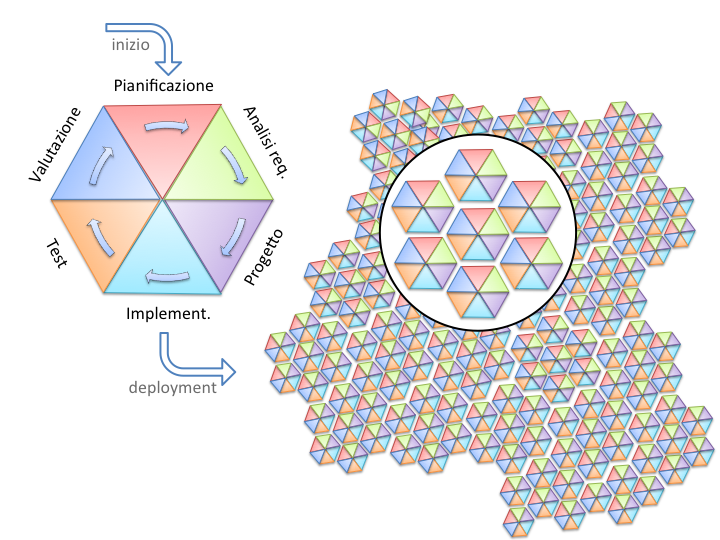
\includegraphics[scale=0.5]{img/modello_incrementale.png}
		\caption{Rappresentazione del modello incrementale \protect\footnotemark}
	\end{figure}

	\footnotetext{Fonte: \url{https://it.wikipedia.org/wiki/Modello_incrementale}}
	